%
% $RCSfile: realisation.tex,v $
%
% Copyright (C) 2002-2008. Christian Heller.
%
% Permission is granted to copy, distribute and/or modify this document
% under the terms of the GNU Free Documentation License, Version 1.1 or
% any later version published by the Free Software Foundation; with no
% Invariant Sections, with no Front-Cover Texts and with no Back-Cover
% Texts. A copy of the license is included in the section entitled
% "GNU Free Documentation License".
%
% http://www.cybop.net
% - Cybernetics Oriented Programming -
%
% http://www.resmedicinae.org
% - Information in Medicine -
%
% Version: $Revision: 1.1 $ $Date: 2008-08-19 20:41:08 $ $Author: christian $
% Authors: Christian Heller <christian.heller@tuxtax.de>
%

\section{Realisation}
\label{realisation_heading}
\index{Res Medicinae Steps of Realisation}

Having analysed the domain of healthcare and having investigated corresponding
standards, actual design solutions that have been tried out in the course of
this work, by implementing them in software source code, can be described in
the following sections.

%
% $RCSfile: student_works.tex,v $
%
% Copyright (C) 2002-2008. Christian Heller.
%
% Permission is granted to copy, distribute and/or modify this document
% under the terms of the GNU Free Documentation License, Version 1.1 or
% any later version published by the Free Software Foundation; with no
% Invariant Sections, with no Front-Cover Texts and with no Back-Cover
% Texts. A copy of the license is included in the section entitled
% "GNU Free Documentation License".
%
% http://www.cybop.net
% - Cybernetics Oriented Programming -
%
% http://www.resmedicinae.org
% - Information in Medicine -
%
% Version: $Revision: 1.1 $ $Date: 2008-08-19 20:41:09 $ $Author: christian $
% Authors: Christian Heller <christian.heller@tuxtax.de>
%

\subsection{Student Works}
\label{student_works_heading}
\index{Res Medicinae Student Works}

Some helpful contributions came from a number of students, collaborating within
the \emph{CYBOP} and/ or \emph{Res Medicinae} projects. The works, completed at
the \emph{Technical University of Ilmenau} (TUI), are of the three types:
\emph{Seminar Paper}, \emph{Research Project} or \emph{Diploma Thesis}, and
listed with their title and results in table \ref{works_table}.

\newpage

The first six of these works were intended to become modules for the first-trial
Java prototype of \emph{Res Medicinae}, as described in the next section.
Further works created tutorials for different base technologies, such as the
\emph{Xlibs} library of the \emph{X Window System} or \emph{Socket Communication}
mechanisms. Finally, one diploma thesis helped in defining the CYBOL language,
by creating a prototype in it.

\begin{table}[ht]
    \begin{center}
        \begin{footnotesize}
        \begin{tabular}{| p{60mm} | p{10mm} | p{35mm} |}
            \hline
            \textbf{Title} & \textbf{Type} & \textbf{Result}\\
            \hline
            A flexible Software Architecture for Presentation Layers demonstrated
            on Medical Documentation with Episodes \cite{bohl}
            & Diploma Thesis & Java application for topological documentation\\
            \hline
            A Technology-neutral Mapping Layer for Data Exchange demonstrated
            on Medical Form Printing as integrative part of an EHR \cite{kunze2003}
            & Diploma Thesis & Java application with one form and persistent storage of data\\
            \hline
            Creating a Backup Module under Consideration of Common Design Patterns
            as provided by the ResMedLib Framework \cite{behrendt}
            & Research Project & Java application for file backup\\
            \hline
            Creating Web Frontends for Scheduling and Management of administrative
            Data, based on a Webserver with JSP Technologie \cite{holzmueller2003}
            & Research Project & Apache webserver extension using Java and JSP\\
            \hline
            Creating Intuitive Frontends under Consideration of
            Internationalisation Aspects \cite{kanagasabapathi}
            & Research Project & Java application in English, German and Tamil (Latha)\\
            \hline
            Evaluating Component Technologies in the Domain of Medical Image Processing \cite{kleinschmidt}
            & Diploma Thesis & ImageJ extension for image transfer via CORBA and SOAP\\
            \hline
            X11 Architecture and XLib Functionality \cite{fache}
            & Seminar Paper & Tutorial and prototype\\
            \hline
            Communication over Sockets \cite{kiesling}
            & Seminar Paper & Tutorial and prototype\\
            \hline
            XML Parser \cite{tellhelm}
            & Seminar Paper & Code fragments\\
            \hline
            Implementation Possibilities for CYBOL Web Frontends, using
            Cybernetics Oriented Programming (CYBOP) Concepts \cite{holzmueller2005}
            & Diploma Thesis & CYBOI extensions and a more detailed CYBOL specification\\
            \hline
        \end{tabular}
        \end{footnotesize}
        \caption{Student Works \cite{cybop}}
        \label{works_table}
    \end{center}
\end{table}

%
% $RCSfile$
%
% Copyright (c) 2005-2006. Christian Heller. All rights reserved.
%
% Permission is granted to copy, distribute and/or modify this document
% under the terms of the GNU Free Documentation License, Version 1.1 or
% any later version published by the Free Software Foundation; with no
% Invariant Sections, with no Front-Cover Texts and with no Back-Cover
% Texts. A copy of the license is included in the section entitled
% "GNU Free Documentation License".
%
% http://www.cybop.net
% - Cybernetics Oriented Programming -
%
% http://www.resmedicinae.org
% - Information in Medicine -
%
% Version: $Revision$ $Date$ $Author$
% Authors: Christian Heller <christian.heller@tuxtax.de>
%

\subsubsection{First Trial}
\label{first_trial_heading}

An early trial of a \emph{Res Medicinae} module was \emph{Record}, an
application for EHR management. It was a standard Java-based system and had a
\emph{Graphical User Interface} (GUI). Its classical architecture made use of
many software patterns and was shared into the parts \emph{Domain Model},
\emph{Graphical View} and \emph{Controller}, as proposed by the equally named
pattern, abbreviated \emph{MVC}.

Later prototypes extended that architecture by applying the CYBOP concept of
\emph{Composition}. In a first step, the \emph{Hierarchical MVC} (HMVC) pattern
was used to replace the MVC pattern, resulting in nested \emph{Controllers} and
\emph{Views}. Afterwards, the principle of \emph{Hierarchy} was applied in
general, also to \emph{Domain Models} and to as many other parts as possible.

Classes as known from \emph{Object Oriented Programming} (OOP) do not represent
dynamically extensible containers but have a static structure with a fixed
number of attributes. In other words, the \emph{Hierarchy} as concept is not
inherent in OOP types. Yet abstract models as humans build them in their minds
are always based on hierarchies (section \ref{reflexions_on_concepts_heading}).
A programming language which does not consider this, does not allow users to
make full use of their modelling potential.

To eliminate this flaw and implement a hierarchical structure in the Java
prototype, a top-most super class named \emph{cybop.Model} had to be introduced.
It represented a container that had the capability to reference itself -- in
other words a \emph{Tree Structure}. As such, it offered \emph{set}, \emph{get}
and \emph{remove} methods for its elements. Since these access methods were
inherited, sub classes did not have to implement their own (for each attribute)
anymore, which saved hundreds of lines of source code.

\begin{figure}[ht]
    \begin{center}
        \includegraphics[scale=0.2]{vector/topological.eps}
        \caption{Topological Documentation}
        \label{topological_figure}
    \end{center}
\end{figure}

One of these advanced modules, to give an example, was responsible for clinical
documentation \cite{hellerbohl}, which it supported graphically, in form of
\emph{Topological Documentation} (figure \ref{topological_figure}). And, of
course, it could also manage and store patient data, in XML files.

%
% $RCSfile$
%
% Copyright (c) 2005-2006. Christian Heller. All rights reserved.
%
% Permission is granted to copy, distribute and/or modify this document
% under the terms of the GNU Free Documentation License, Version 1.1 or
% any later version published by the Free Software Foundation; with no
% Invariant Sections, with no Front-Cover Texts and with no Back-Cover
% Texts. A copy of the license is included in the section entitled
% "GNU Free Documentation License".
%
% http://www.cybop.net
% - Cybernetics Oriented Programming -
%
% http://www.resmedicinae.org
% - Information in Medicine -
%
% Version: $Revision$ $Date$ $Author$
% Authors: Christian Heller <christian.heller@tuxtax.de>
%

\subsubsection{Knowledge Separation}
\label{knowledge_separation_heading}

In the case of the first prototypes, one could still speak of true
\emph{Implementation}, because design models had to be transferred into another
form of abstract model: the Java programming language source code. Not so in
later versions of \emph{Res Medicinae}.

While the early prototypes represented the classical mix of domain knowledge
and low-level system instructions, that was eliminated later. All knowledge got
\emph{extracted} and was put into special configuration files, in \emph{CYBOL}
format (section \ref{cybol_heading}). Henceforth, these contained not only
settings like font size or colour, as known from standard applications, but the
\emph{whole} domain knowledge, including user interface- and workflow structures.

Following the explanations of section \ref{state_and_logic_heading}, the
\emph{static} knowledge was shared into different models, some representing
\emph{state-}, and others \emph{logic} knowledge. This was very much opposed to
the earlier Java implementations whose classes bundled attributes and methods.

Without the knowledge, the remaining program code looked pretty much like a
skeleton of basic system functionality. Serving as hardware interface, it
concentrated memory- and signal handling in one place -- exactly those things
which section \ref{statics_and_dynamics_heading} called \emph{Dynamics}.
Additionally, that remaining system had the ability to interpret knowledge,
which is why it was called \emph{CYBOI} (interpreter). One could, in some way,
compare it with what the \emph{Java Virtual Machine} (JVM) is for Java, only
that CYBOI processed knowledge given in form of CYBOL templates, which look
different than Java source code.

CYBOI needed an \emph{XML Parser} in order to be able to read the knowledge
contained in CYBOL files. The decision here fell on Apache's \emph{Xerces}
\cite{xerces}, because one of its versions is implemented in Java.

%
% $RCSfile: reimplementation.tex,v $
%
% Copyright (C) 2002-2008. Christian Heller.
%
% Permission is granted to copy, distribute and/or modify this document
% under the terms of the GNU Free Documentation License, Version 1.1 or
% any later version published by the Free Software Foundation; with no
% Invariant Sections, with no Front-Cover Texts and with no Back-Cover
% Texts. A copy of the license is included in the section entitled
% "GNU Free Documentation License".
%
% http://www.cybop.net
% - Cybernetics Oriented Programming -
%
% http://www.resmedicinae.org
% - Information in Medicine -
%
% Version: $Revision: 1.1 $ $Date: 2008-08-19 20:41:08 $ $Author: christian $
% Authors: Christian Heller <christian.heller@tuxtax.de>
%

\subsection{Reimplementation}
\label{reimplementation_heading}
\index{CYBOP}
\index{Itemisation}
\index{Composition}
\index{Bundling of Attributes and Methods}
\index{Container Inheritance}
\index{CYBOL}
\index{CYBOI}
\index{OOP}
\index{Java Programming Language}
\index{C++ Programming Language}
\index{C Programming Language}
\index{Operating System}
\index{OS}
\index{XML}
\index{Graphical User Interface}
\index{GUI}
\index{empty}
\index{Abstract Windowing Toolkit}
\index{AWT}
\index{Swing}
\index{Qt}
\index{wxWindows}
\index{Gimp Toolkit}
\index{GTK}
\index{GNU/Linux}
\index{XFree86}
\index{X-Library}
\index{Xlib}
\index{Textual User Interfaces}
\index{TUI}
\index{Web User Interfaces}
\index{WUI}
\index{Socket Communication Mechanisms}

The architecture-advanced prototype of the \emph{Record} module had \emph{much}
less functionality than earlier ones, in fact not much more than starting a
graphical frame with menu bar and exiting the application again. This was so,
because yet before all domain knowledge could be extracted into CYBOL, another
issue turned up:

CYBOP modelling concepts like \emph{Itemisation} or \emph{Composition} are an
integral part of the CYBOL knowledge representation language. Other concepts
like the \emph{Bundling} of attributes and methods, property- and container
\emph{Inheritance}, as known from \emph{Object Oriented Programming} (OOP),
were considered unfavourable (section \ref{object_oriented_programming_heading})
and neither to be used in CYBOL, nor in the CYBOI interpreter. Consequently,
OOP languages like Java or C++ were not suitable for CYBOI any longer. A slim
and fast language, close to hardware and fast in processing CYBOL was needed.

Having such requirements, one of the first candidates coming to mind was the
\emph{C} programming language. It is \emph{high-level} enough to permit fast
programming and \emph{low-level} enough to connect efficiently to hardware or
an \emph{Operating System} (OS). Many OS are written in C themselves, anyway.
CYBOI was therefore reimplemented in C, which hasn't changed since. What has
changed and is changing all the time is its functionality, an overview of which
was given in chapter \ref{cybernetics_oriented_interpreter_heading}.

CYBOL sticks to the XML specification and standard XML parsers can be used to
process and validate it. However, for reasons of performance and better
integration, and due to the very limited vocabulary (set of possible tags and
attributes), special parsing procedures were written and adapted to CYBOI.

Another problem that had to be solved was \emph{Graphical User Interface} (GUI)
handling. While the Java-implemented CYBOI could make use of the
\emph{Abstract Windowing Toolkit} (AWT)/ Swing, the C-implemented CYBOI did not
have such functionality at first. Toolkit candidates like \emph{Qt} \cite{qt}
or \emph{wxWindows} \cite{wxwidgets}, being implemented in C++, were out. Other
GUI frameworks like the \emph{Gimp Toolkit} (GTK) \cite{gtk}, written in C,
were considered cumbersome to cope with so that finally, the decision was taken
to use low-level graphics drawing routines. For CYBOI, being developed on a
\emph{GNU/Linux} OS \cite{linux}, that meant using \emph{XFree86's}
\cite{xfree86} \emph{X-Library} (Xlib) functionality directly. The necessary
effort for transforming hierarchical CYBOL models into GTK- or other toolkit
structures was estimated to be equal or even higher than translating them into
Xlib functionality right away. At the time of writing this work, implementation
is in progress but not completed.

Similar implementations are necessary for \emph{Textual User Interfaces} (TUI),
\emph{Web User Interfaces} (WUI) and \emph{Socket Communication Mechanisms},
the latter two being already finished in a first version. Further development
activities may for instance enable CYBOI to run on other platforms and integrate
more hardware-driving functionality, to get independent from underlying OS.

While the CYBOL specification can be considered quite mature, CYBOI, as could
be seen, will need plenty of extensions and additions in future, in order to
leave its prototype stage and become fully usable.

%
% $RCSfile$
%
% Copyright (c) 2005-2006. Christian Heller. All rights reserved.
%
% Permission is granted to copy, distribute and/or modify this document
% under the terms of the GNU Free Documentation License, Version 1.1 or
% any later version published by the Free Software Foundation; with no
% Invariant Sections, with no Front-Cover Texts and with no Back-Cover
% Texts. A copy of the license is included in the section entitled
% "GNU Free Documentation License".
%
% http://www.cybop.net
% - Cybernetics Oriented Programming -
%
% http://www.resmedicinae.org
% - Information in Medicine -
%
% Version: $Revision$ $Date$ $Author$
% Authors: Christian Heller <christian.heller@tuxtax.de>
%

\subsubsection{Module Modelling}
\label{module_modelling_heading}

When CYBOI had become more stable (besides the extensions that were -- and are
-- frequently implemented, development could focus on the actual application
again. From now on, \emph{Res Medicinae} modules only had to be \emph{modelled}
in CYBOL, but no longer had to be \emph{coded} in a programming language. The
designed state- and logic knowledge, existing in form of CYBOL templates,
already represented the complete application; no further implementation phase
was needed.

\begin{figure}[ht]
    \begin{center}
        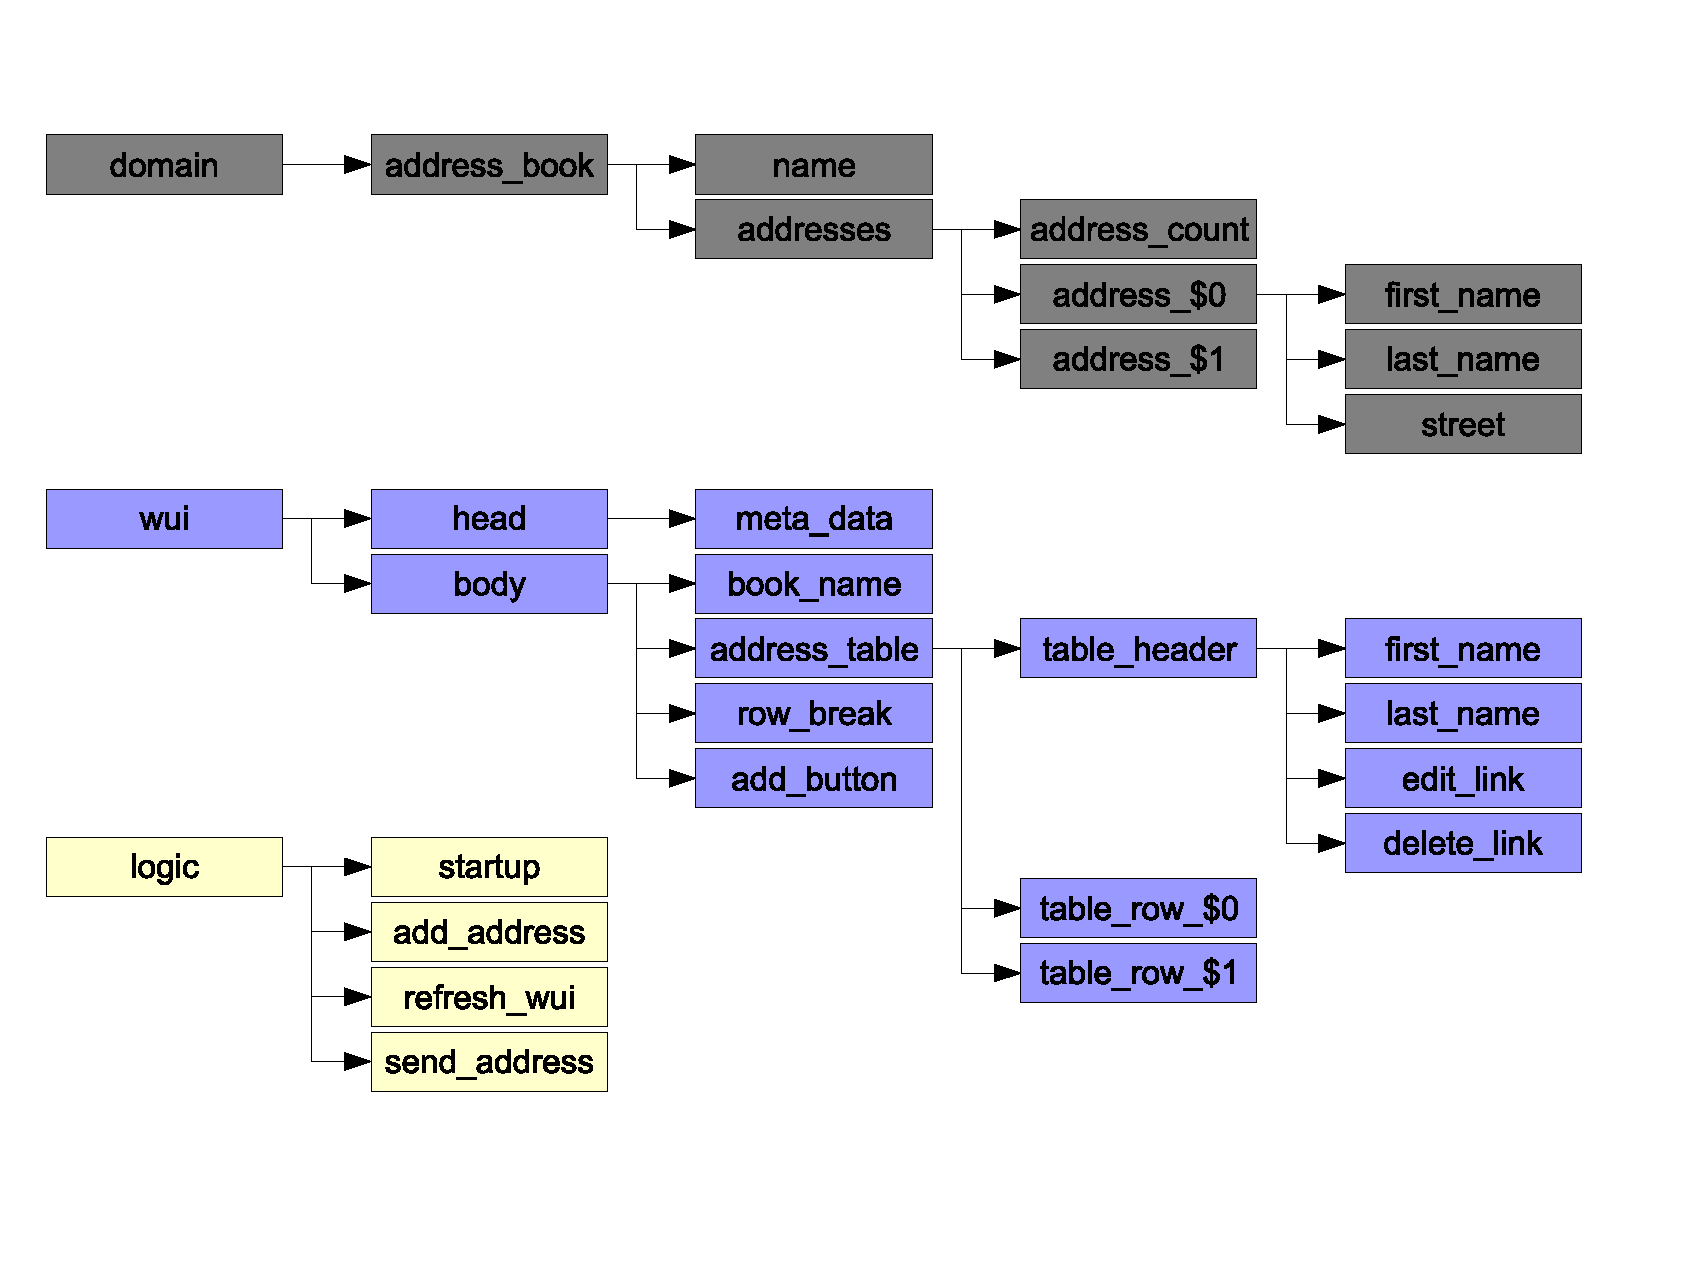
\includegraphics[scale=0.2]{vector/radesign.eps}
        \caption{ResAdmin Knowledge Models}
        \label{radesign_figure}
    \end{center}
\end{figure}

Due to the tremendous complexity of an \emph{Electronic Health Record} (EHR),
only a very small part of its data could be considered for the application
prototype. Administrative data like a person's name or address are standard
information found in all EHRs. A corresponding module named \emph{ResAdmin}
\cite{holzmueller2005} was therefore elected to be realised first. Its models
belong to three categories: \emph{Domain}, \emph{Web User Interface} (WUI) and
\emph{Logic} (figure \ref{radesign_figure}).

The addresses contained in the \emph{domain} branch of the knowledge tree are
manipulated across \emph{Hyper Text Markup Language} (HTML) \emph{User Interface}
(UI) models belonging to the \emph{web} branch of that same tree. An example
structure of a knowledge tree was shown in figure \ref{mvctree_figure}. Every
action model that a user can trigger through the WUI exists as part of the
\emph{logic} branch of the knowledge tree.

Independently of what kind of knowledge model (state or logic) was created,
ontological principles were strictly followed. Most importantly, relations
within a hierarchical model were always \emph{unidirectional}, that is from a
\emph{Whole-} to its \emph{Part} models, but never the other way around.
Additionally, however, logic models may reference and access runtime state
models.

Some of the logic models represent \emph{Translators} (compare section
\ref{communication_model_heading}). They extract address information
residing in the domain- and copy them to the web model, which is afterwards
sent to the human user as communication partner. This principle holds true for
the communication between application systems, only that then other than web
models are used as communication format. The vision to make all communication
channels really \emph{transparent} and easy to handle for the user now seems to
be coming true.

